\documentclass[letterpaper,10pt]{article}
\usepackage[top=2cm, bottom=1.5cm, left=1cm, right=1cm]{geometry}
\usepackage{amsmath, amssymb, amsthm,graphicx}
\usepackage{fancyhdr}
\pagestyle{fancy}

\lhead{\today}
\chead{MATH 710 Assignment 4}
\rhead{Justin Hood}

\newcommand{\Z}{\mathbb{Z}}
\newcommand{\Q}{\mathbb{Q}}
\newcommand{\R}{\mathbb{R}}
\newcommand{\C}{\mathbb{C}}
\newtheorem{lem}{Lemma}

\begin{document}
\begin{enumerate}
\item We consider the equation in Meyer's text,
\[\frac{dx}{dt}=s\bigg(1-\frac{x}{K}\bigg)x\]
\begin{enumerate}
\item We begin by expanding and manipulating the above equation into the following form,
\[\frac{dx}{dt}-sx=-\frac{s}{K}x^2\]
We note the form of the Bernoulli equation,
\[\frac{dx}{dt}+p(t)x=q(t)x^n\]
As such, we see $n=2$, $p(t)=-s$, and $q(t)=-\frac{s}{K}$.
\item We now make the following substitution,
\begin{align*}
v &= x^{-1}\\
\Rightarrow \frac{dv}{dx} &= -x^{-2}\frac{dx}{dt}\\
\Leftrightarrow -x^2\frac{dv}{dx} &= \frac{dx}{dt}
\end{align*}
Thus, we may manipulate the original equation,
\begin{align*}
\frac{dx}{dt}+(-s)x &= (-\frac{s}{K})x^2\\
\frac{1}{x^2}\frac{dx}{dt}+(-s)x^{-1} &= -\frac{s}{K}\\
-\frac{dv}{dt}+(-s)v &= -\frac{s}{K}\\
\frac{dv}{dt}+sv &= \frac{s}{K}
\end{align*}
Which is now in a linear form.
\item We will now use the method of integrating factors to solve the equation. Consider,
\[\mu=e^{\int p(t)dt}=e^{\int sdt}=e^{st+c_1}=c_1e^{st}\]
We then multiply through the linear ODE by $\mu$.
\[c_1e^{st}\frac{dv}{dt}+c_1se^{st}v=\frac{s}{K}c_1e^{st}\]
We note that the left hand side of the equation may be considered as $\frac{d}{dt}(c_1e^{st}v)$ Thus, we may integrate with respect to $t$ and arrive at,
\begin{align*}
\int \frac{d}{dt}(c_1e^{st}v)dt &= \int \frac{s}{K}c_1e^{st} dt\\
\Rightarrow c_1e^{st}v &= \frac{c_1}{K}e^{st}+c_2
\end{align*}
Dividing by our constant, we see,
\[e^{st}v=\frac{1}{K}e^{st}+C\]
Dividing again,
\[v=\frac{1}{K}+Ce^{-st}\]
\item Recall that $v=x^{-1}$. Thus,
\begin{align*}
x^{-1} &= \frac{1}{K}+Ce^{-st}\\
x^{-1} &= \frac{KC+e^{st}}{Ke^{st}}\\
x &= \frac{Ke^{st}}{KC+e^{st}}
\end{align*}
\item Finally, we consider the relation,
\[1=\frac{e^{-st}}{e^{-st}}\]
Thus,
\[\frac{Ke^{st}}{KC+e^{st}}\frac{e^{-st}}{e^{-st}}=\frac{K}{Ce^{-st}+1}\]
Thus, we finally arrive at the solution to the differential equation,
\[x(t)=\frac{K}{Ce^{-st}+1}\]
\end{enumerate}
\item We now perform some analysis on the equation from above,
\[\frac{dx}{dt}=s\bigg(1-\frac{x}{K}\bigg)x\]
\begin{enumerate}
\item First, we compute the equilibrium points, by solving the equation,
\[s\bigg(1-\frac{x}{K}\bigg)x=0\]
It is trivial to see that the solutions to this equation are $x=0,K$. Thus, our equation has two equilibrium points. Next, we shall analyze the stability of these equilibrium points by looking at the following equalities regarding values of the population within each of the realms of the solution space,
\begin{align*}
x<0 &\Rightarrow \frac{dx}{dt}<0\\
0<x<K &\Rightarrow \frac{dx}{dt}>0\\
x>K &\Rightarrow \frac{dx}{dt}<0
\end{align*}
Thus, we see that the equilibrium point at $x=K$ is stable, and the point at $x=0$ is unstable. So, we consider a toy problem with $s=.3$ and $K=5$. We expect to see two different equilibrium points, one at $x=0$ and $x=5$. We also expect to see the slopes for each of the regions of the phase plane to follow the slope equalities above. After performing the computations for the phase plane, we arrive at the following,
\begin{center}
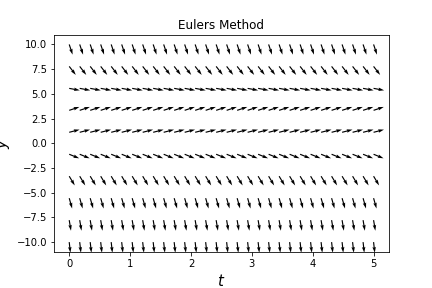
\includegraphics[scale=1]{2a.png}
\end{center}
We see that the behavior is as we would expect. Next, we will use the Forward Euler Method to compute three solutions of the toy problem numerically in order to analyze the stability of the solutions. We take the three initial conditions $x_0=-1,1,7$
\begin{center}
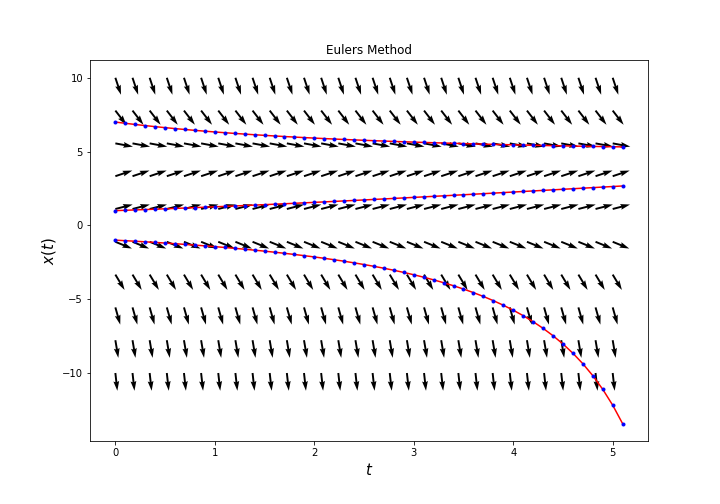
\includegraphics[scale=.7]{2b.png}
\end{center}
We see that the solutions tend towards and away from the equilibrium points as we expect.
\item We will now solve to find the point where the rate of growth is maximal.\\
Note that our original differential equation defines the rate of growth of the population $x$. Thus, we shall derive the equation with respect to $x$ to find the critical values of the equation. So,
\begin{align*}
\frac{dx}{dt} &= sx-\frac{s}{K}x^2\\
\frac{d^2x}{dt^2} &= s-\frac{2s}{K}x
\end{align*}
Setting this equal to $0$ and solving for $x$,
\begin{align*}
0 &= s-\frac{2s}{K}x\\
\frac{2s}{K}x &= s\\
\Rightarrow \frac{2}{K}x &= 1\\
\Rightarrow x &= \frac{K}{2}
\end{align*}
Because this is the only solution to this equation, we know that it maximizes the population rate of change. So, we see that the population rate of change is greatest when it is half of the population cap.
\end{enumerate}
\end{enumerate}
\end{document}
